\documentclass{article}
\usepackage{graphicx}
\usepackage{float}

\title{Note on [Learning to Edit: Aligning LLMs with Knowledge Editing]}
\author{NoteAuthor: XIONG ZHIPENG}
\date{\today}

\begin{document}


\maketitle

\section{Which problem is addressed by the paper?}
Efficiently modify LLMs' outputs towards targeted queries while preserving overall performance across other unrelated ones

\textbf{For example:}
updating the knowledge of "\textit{The current British Prime Minister is Rishi Sunak}" 
modifies the response to "\textit{Who is married to the PM of the UK?}" 



\section{Why is it important?}

The dynamic nature of the world  necessitates frequent updates to LLMs to rectify outdated information 
or integrate new knowledge, thereby safeguarding their sustained pertinence.

This paper argues that the previous methods predominantly rely on memorizing 
the update.



\begin{figure}[H]
    \centering
    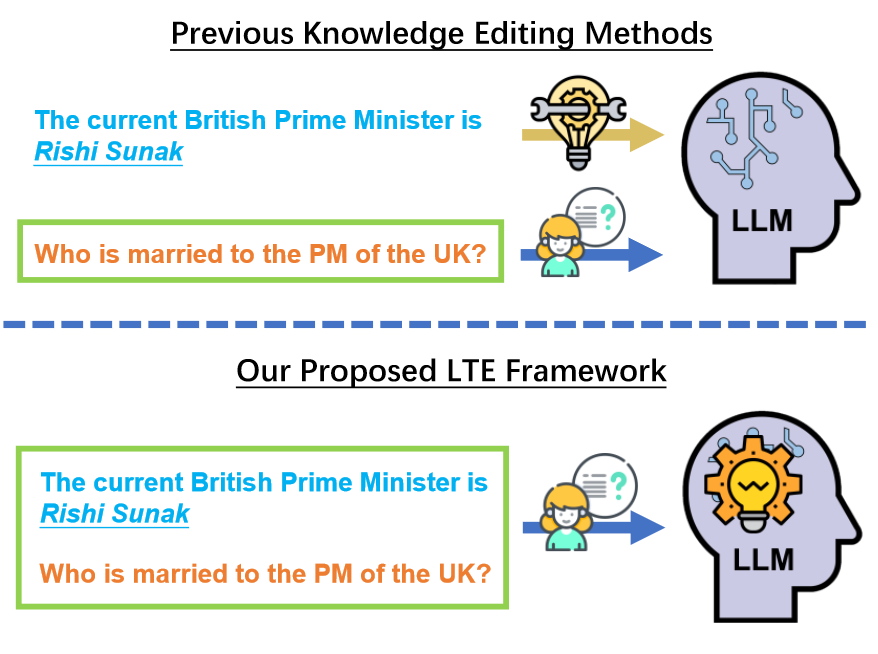
\includegraphics[width=\textwidth]{./../Images/Figure1.png}
    \caption{The previous and proposed principles}
\end{figure}

\section{How is it solved?}
\textbf{Two phases}
\begin{itemize}
    \item \textbf{Alignment Phase:} train LLMs how to apply updated knowledge
    \item \textbf{Inference Phase:} propose a retrieval-based mechanism that retrieves relevant edit descriptors from a stored memory for real-time, mass editing requests.
\end{itemize}

\begin{figure}[H]
    \centering
    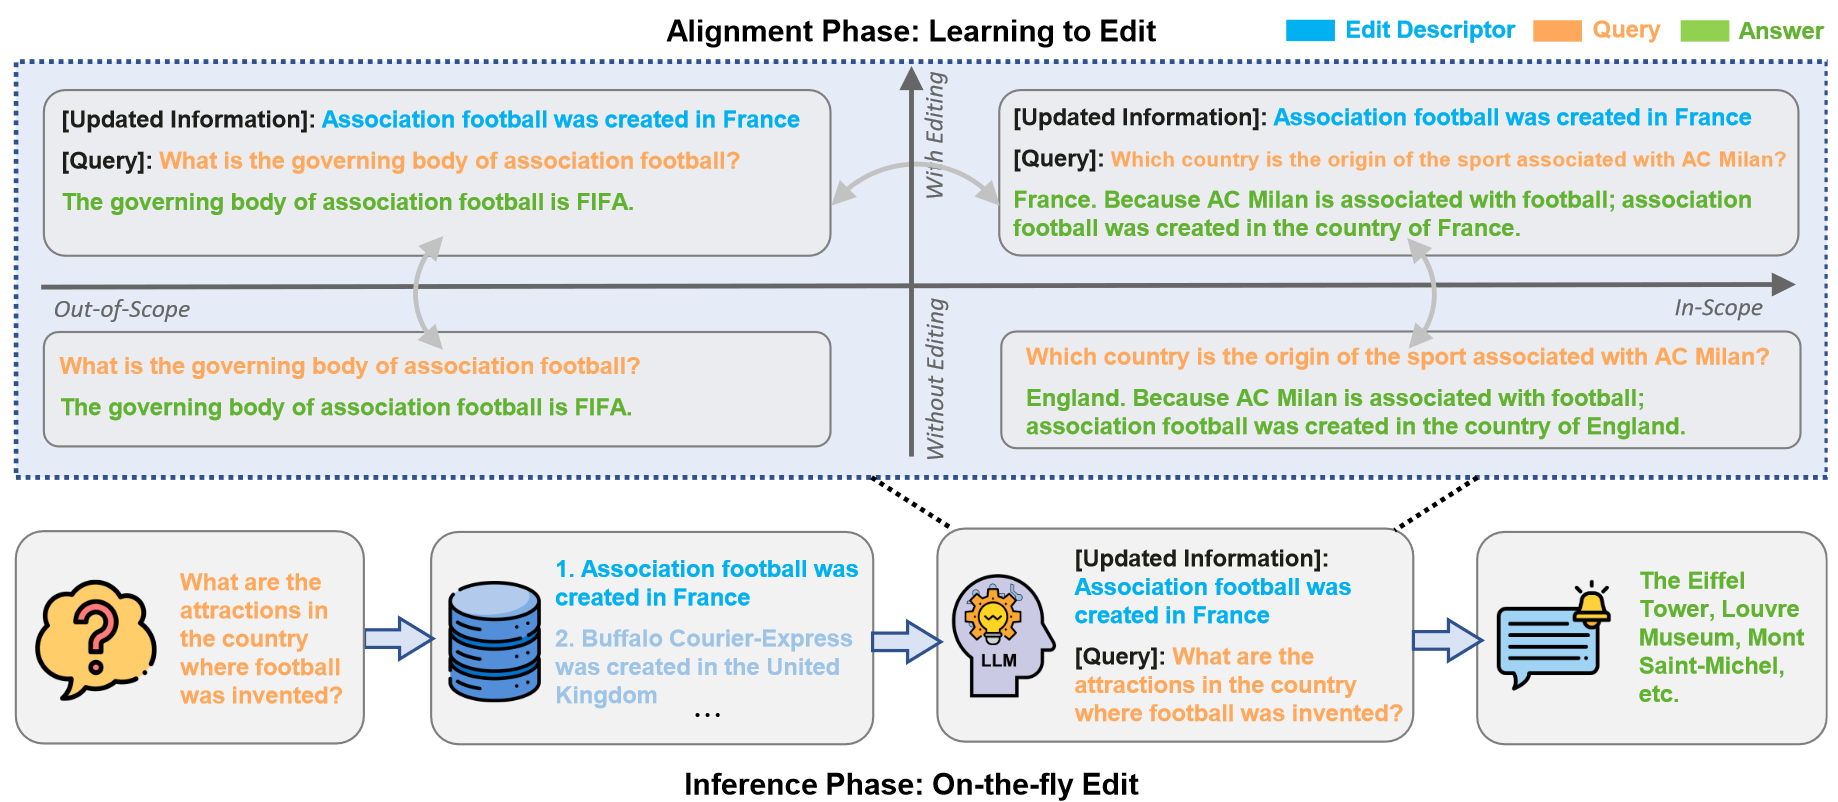
\includegraphics[width=\textwidth]{./../Images/Figure2.png}
    \caption{The proposed feamework}
\end{figure}


\section{DataAnalysis, Applications, Conclusion and Future Work}


\end{document}